\maketitle

\begin{abstract}
Since the beginning of AI research, the study on one of its core
component, graph search, has long focused on how to guide it using the
heuristic estimate and how to improve the estimates.  One thing that has
been out of focus is the study on tiebreaking, or how to \emph{directly}
improve the search performance on a plateau without changing the
heuristics nor search algorithms.  Such techniques should be done
without help of additional information from the heuristics because
theoretically there is some point that the heuristics cannot be improved
any more while the plateau is still exponentially large.

In this paper, we investigate and improve tiebreaking strategies for
 optimising search using A* and satisficing search using GBFS.
For A*, we first experimentally analyze the performance of common tiebreaking strategies that break ties according to the heuristic value of the nodes.
We find that tiebreaking has a significant impact on search algorithm performance when there are zero-cost operators that induce large plateau regions in the search space.
Next we develop a new framework for tiebreaking based on a depth metric which
 measures the distance from the entrance to the plateau, and propose a new, diversifying strategy which significantly outperforms standard strategies on domains with zero-cost actions. 

We also apply the same strategy to GBFS for satisficing search, where
 currently no obvious tiebreaking rules are proposed. Our depth
 diviersification resulted in an improvement orthogonal to the other
 search enhancements such as Lazy Evaluation, Preferred Operators,
 Multi-heuristic search, and recently proposed Type-Based
 diversification tequeniques.

Finally, we provide a theoretical analysis on why the depth-based
diversification improves the performance of several algorithms. By doing
this, it ensure the same technique can applied to various best first
search algorithms that are not investigated in this paper such as
Weighted A*.

This paper is a significantly extended version of the AAAI-16 paper by
the same authors.
\end{abstract}

\section{Introduction}
\label{sec:introduction}

Much of the work in the search and planning literature has focused on
reducing the size of this effective search space by developing the more
informative heuristic functions. However, there is a theoretical
limitation in this approach: It is known that the search space grows
exponentially \cite{helmert2008good} even under the optimistic
assumption that we have an \emph{almost-perfect} heuristics, $h^*-c$, a
theoretical heuristic function which always returns an estimate which is
slightly underestimates the true distance to a goal by a small constant
$c$. Due to this, the community recognizes the importance of developping
a heuristic-agnostic improvement which can overcome this difficulty.

As an instance of such improvement, this paper investigates tiebreaking
strategies for search algorithms. We empirically and theoretically
analyse both optimal and satisficing search.

\subsubparagraph{astar}

From \refsec{sec:astar-background} to \refsec{sec:depth}, we investigate
the tiebreaking strategy used by \astar, the standard search algorithm
for finding an optimal-cost path from an initial state $s$ to some goal
state $g \in G$ in a search space represented as a graph
\cite{hart1968formal}. 

In many problems, the size of the last layer of search, called
\emph{final plateau}, accounts for a significant fraction of
the effective search space of \astar.  \refig{fig:plateau-noh}
(\refpage{fig:plateau-noh}) plots the
number of states with $f(n) = f^*$ (y-axis) vs. the number of states with
$f(n) \leq f^*$ for 1104 problem instances from the International
Planning Competition (IPC1998-2011).  For many instances, a large
fraction of the nodes in the effective search space have $f(n)=f^*$.
In many domains, the points are located very close to the diagonal $x=y$
line, indicating almost all states with $f(n) \leq f^*$ have cost $f^*$.
% For example, in the \pddl{Openstacks} domain, almost all states with
% $f(n) \leq f^*$ have cost $f^*$ due to the large number of actions with
% cost 0.


% In many problems, the size of the last layer of search (which explores
% the set of nodes with $f(n)=f^*$) accounts for a significant fraction of
% the effective search space of \astar.  \refig{fig:plateau-noh}
% (\refpage{fig:plateau-noh}) plots the
% number of states with $f(n) = f^*$ (y-axis) vs. the number of states with
% $f(n) \leq f^*$ for 1104 problem instances from the International
% Planning Competition (IPC1998-2011).  For many instances, a large
% fraction of the nodes in the effective search space have $f(n)=f^*$.
% For example, in the \pddl{Openstacks} domain, almost all states with
% $f(n) \leq f^*$ have cost $f^*$ due to the large number of actions with
% cost 0.

\begin{figure}[htbp]
  \centering
  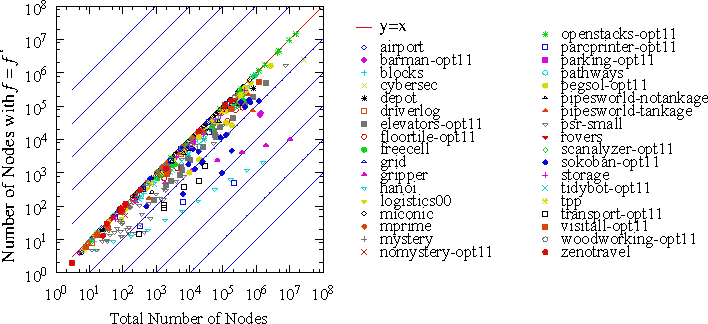
\includegraphics{tables/aaai16-frontier/aaai16prelim3/lmcut_frontier_noh-front.pdf}
 \caption{
 The number of nodes with $f=f^*$ (y-axis) compared to the
 total number of nodes in the search space (x-axis) with $f\leq f^*$ on 1104 IPC benchmark problems,
  using modified Fast Downward with \lmcut which 
  generates all nodes with cost $f^*$.
  }
 \label{fig:plateau-noh}
\end{figure}

Therefore, in those majority of IPC problem instances where the size of
the last layer ($f(n)=f^*$) of search is huge, a
\emph{tiebreaking policy} can have a significant impact on the
performance of \astar. Tiebreaking policy is a policy 
for selecting which node to expand among nodes with the same $f$-cost.
It is widely believed that among nodes with the same $f$-cost,
ties should be broken according to $h(n)$, i.e.,
nodes with smaller $h$-values should be expanded first.  While this is a
useful rule of thumb in many domains, it turns out that tiebreaking
requires more careful consideration, particularly for problems where
this tiebreaking does not reduce the size of the plateau.

We first empirically evaluate the existing, commonly used, standard
tiebreaking strategies for \astar.
In the experiments, we show that:
\begin{enumerate}
 \item Last-In-First-Out (\lifo) policy tends to be more efficient
       than a First-In-First-Out (\fifo) policy.
 \item Tiebreaking according to the heuristic value $h$, which
       frequently appears in the heuristic search literature, has little
       impact on the performance as long as a \lifo policy is used.
 \item There are significant performance differences among tiebreaking strategies
       when domains include zero-cost actions.
\end{enumerate}
While there are relatively few domains with zero-cost actions in the
IPC benchmark set, we argue that zero-cost actions naturally occur in 
practical cost-minimization problems.

In order to solve such problems more efficiently, we propose a new
tiebreaking method based on a notion of \emph{depth} within the plateau,
corresponding to the number of steps a node is from the ``entrance'' to
the plateau.  We empirically show that:
\begin{enumerate}
 \item Depth-based diversification strategy significantly outperforms
       other tiebreaking strategies using the same heuristic function.
 \item Artificial gradient introduced by $\epsilon$-cost conversion or
       PLUS\-ONE cost types does not achieve the performance better than
       our strategy.
 \item $\epsilon$-cost and PLUS\-ONE cost types essentially makes the
       task computationally harder in the context of cost-optimal
       planning, while depth-based diversification does not.
\end{enumerate}

Note that all tiebreaking strategies in this section maintain the
optimality of the search algorithm because they only affect node
expansion order among the nodes with the same $f$-cost.

\subsubparagraph{gbfs}

After \refsec{sec:gbfs}, we apply the same depth-based diversifying tiebreaking
method to Greedy Best First Search (GBFS) for satisficing planning.

Despite the ubiquitous use of GBFS for satisficing search,
various research have suggested that GBFS can be
easily trapped by undetected dead ends and a huge search plateau.
On infinite graphs, GBFS is not even complete \cite{Valenzano2016}
because it can be misdirected by the heuristic guidance forever.
These pathological behaviors are caused by the fact that 
the search process of GBFS heavily relies upon the
quality of the heuristic function.

The problem is amplified by the fact that GBFS is usually combined
with inadmissible heuristic functions, such as FF
heuristics\cite{Hoffmann01}, Causal Graph heuristics \cite{Helmert2006}, Context Enhanced
Additive (CEA) heuristics\cite{helmert2008unifying}.
% , Landmark-count heuristics\cite{richter2008landmarks}
These functions may overestimate the true distance to the goal,
which can causes some important nodes to be incorrectly labelled as unpromising
(very far from the goal). Best-first search algorithms like GBFS thus
ignores these nodes until after expanding all other nodes with the smaller estimates.

Recently, several approaches
\cite{imai2011novel,valenzano2014comparison,xie14type} have been
proposed for alleviating those problems in GBFS. They improve the search
performance by occasionally ignoring the heuristic guidance, which
provides a chance to recover from the past wrong decisions made by the
heuristics, and makes the algorithm more robust against the heuristic
errors.  These diversified algorithms are probabilistically complete on
the inifinite graphs \cite{Valenzano2016}: The probability of finding a
solution approaches to 1 as the runtime approaches to infinity; in other
words, it eventually finds a solution.

% by relaxing its dependency to the heuristic function.

%% this paragraph is important because diversity, exploration, and
%% ``removing bias'' might not immediately connect with each other
One common theme in these algorithms is to remove the \emph{bias} and
add a \emph{diversity} and \emph{exploration} to the search process.
Exploration, an opposite word to exploitation, is an act of removing
the focus or the bias, thus is equivalent to an act of introducing the
diversity. Hereafter, we use these three key words interchangeably.

In these sections, we show that there is much more room for diversifying
the behavior of GBFS, and show that the use of our depth-based
tiebreaking strategy improves the performance of GBFS by
diversifying the search within the same $h$-plateau.
 
GBFS variants mentioned above all employ the exploration by occasionally
expanding the nodes with bad heuristic estimates. While this can avoid
the problem of large bias of the search algorithm to the nodes with the
least estimates, it cannot detect the bias among the nodes with the
\emph{same} estimates. Imagine what happens if a heuristic function
always returns a constant value $c$. Since all nodes expanded by GBFS
has the same evaluation $c$, above-mentioned GBFS variants fail to
identify their difference based on the estimates. \footnote{Type-GBFS
and DBFS2 can also diversify the search based on the $g$ value, the
current shortest path cost from the initial state.}

To our knowledge, there are currently no well-established tiebreaking
policy for GBFS.  Compared to \astar, GBFS does not use $f$ and $g$
value during the search process.  The search by GBFS is solely guided by
the heuristic value $h$: It always expands the node with the smallest
$h$ value, and hence the analogy from \astar e.g.\ sorting the nodes
with $f$ and breaking ties according to $h$ is not possible.

% We propose the use of recently proposed tiebreaking strategy based on
% the \emph{depth} of each node from the entrance in the plateau, originally
% designed for \astar, also improves the performance of GBFS by
% diversifying the search within the same h-plateau.
Our depth-based tiebreaking can be implemented as an extension to GBFS, and
can also be incorpolated as a part of type-bucket generation criteria in
Type-Based GBFS.  We empirically evaluate the performance of the
proposed approach, comparing numerous search enhancement techniques such
as Lazy Evaluation, PLUS\-ONE/ONE cost type, Preferred Operators and
Multi-queue heuristic search.
